\section*{Appendix}
\subsection{regulation document}
\label{sec:appendix}

\label{sec:regulation_document}
Regulation1: 
\begin{figure}
    \centering
    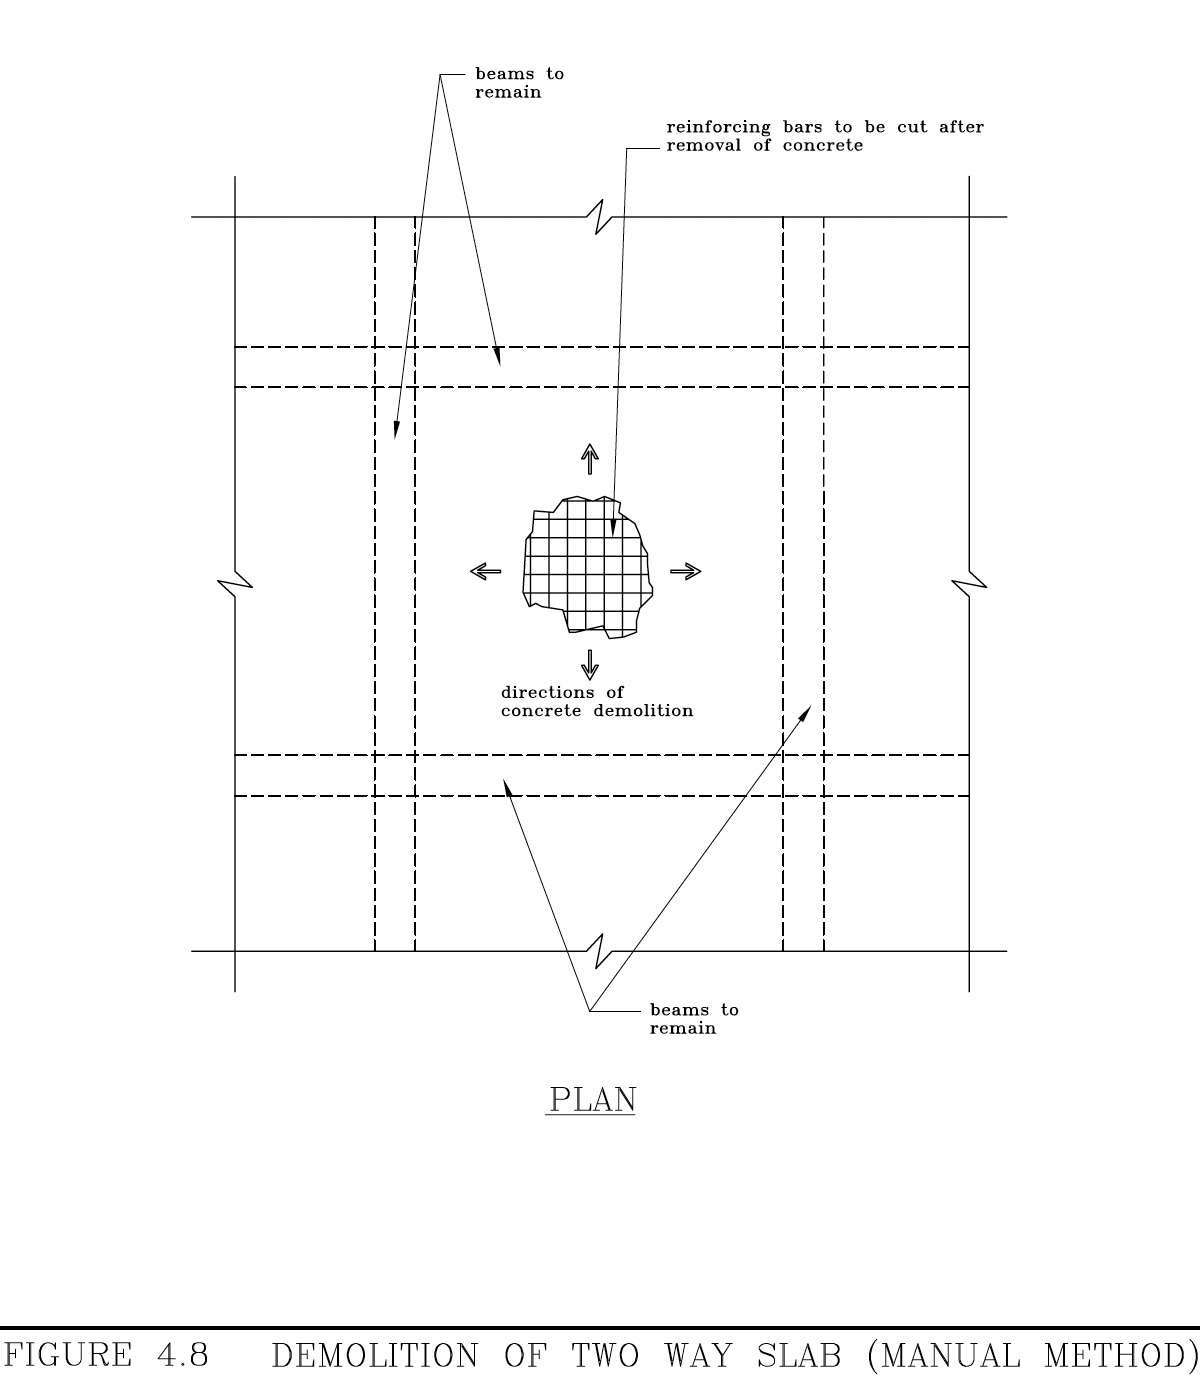
\includegraphics[width=0.5\textwidth]{figures/Demolition-of-Two-way-slab.jpeg}
    \caption{Regulation1}
    \label{fig:regulation1}
\end{figure}
Regulation2: 
\begin{figure}
    \centering
    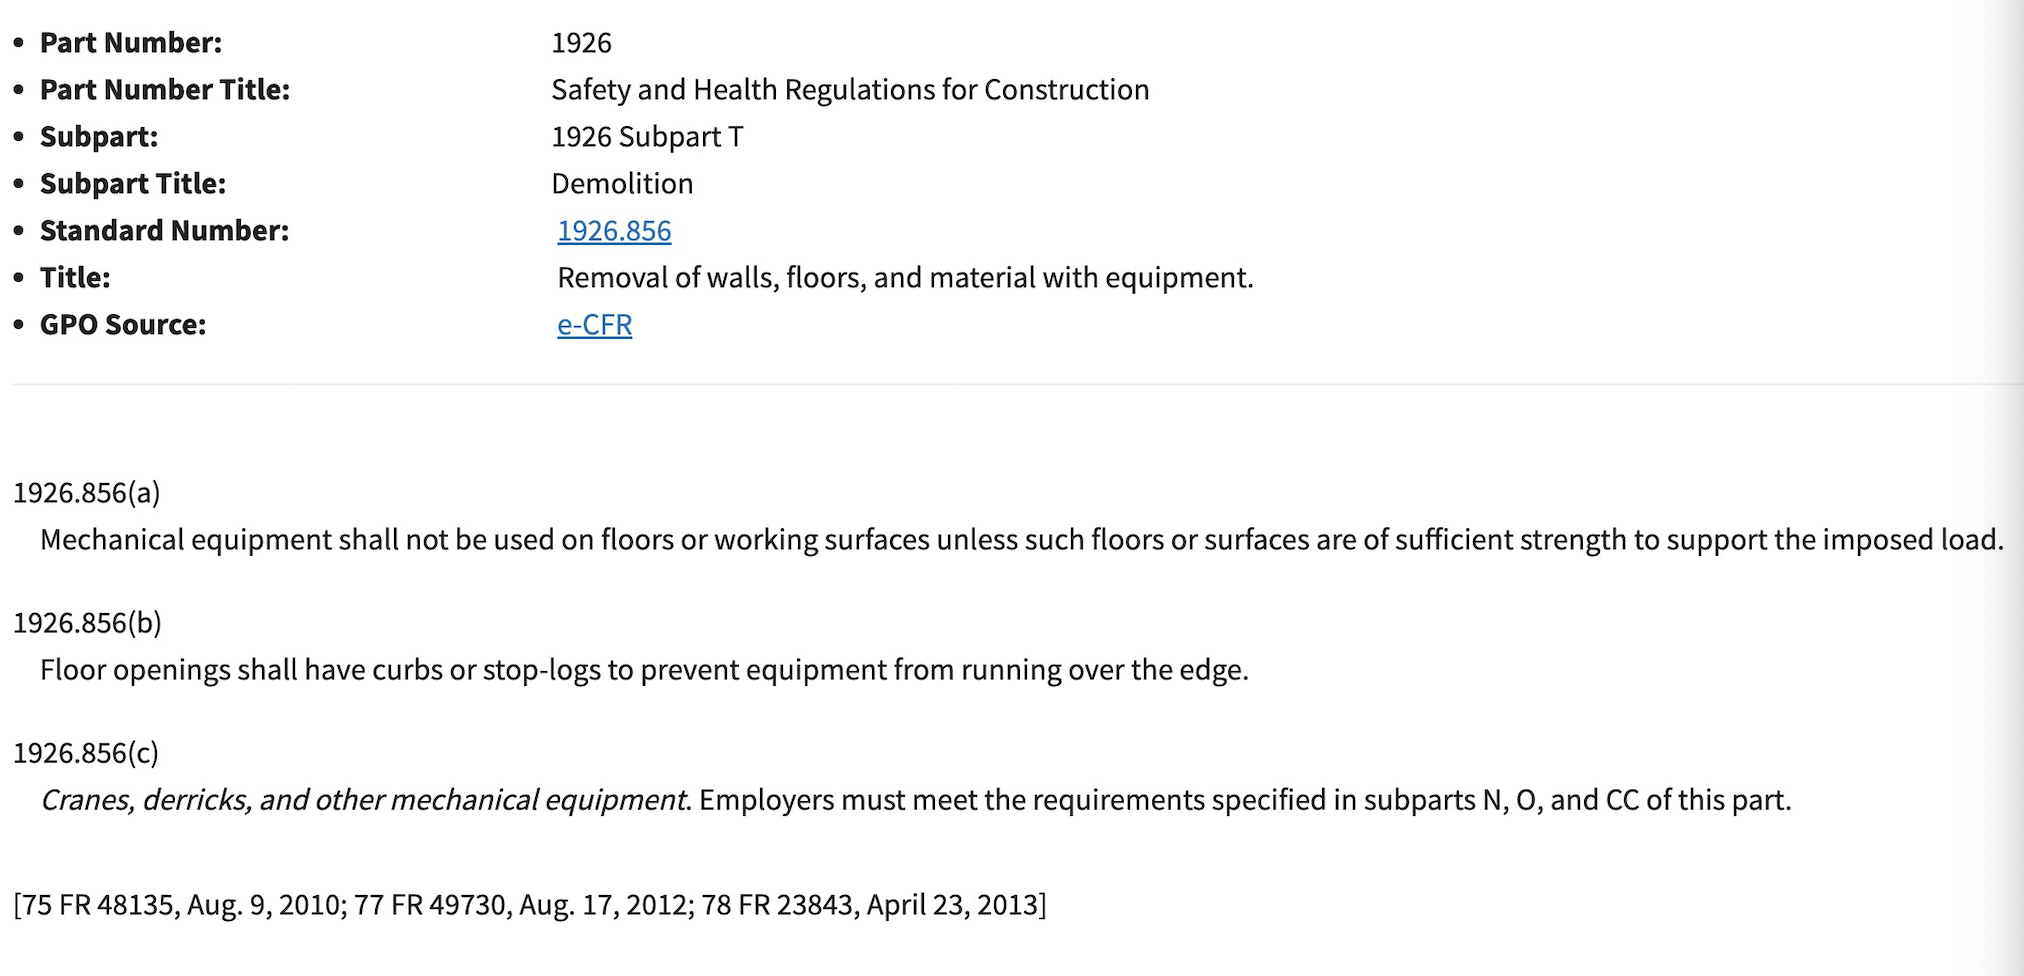
\includegraphics[width=0.5\textwidth]{figures/Removal-of-walls-floors-and-material-with-equipment.png}
    \caption{Regulation2}
    \label{fig:regulation2}
\end{figure}
Regulation3: 
\begin{figure}
    \centering
    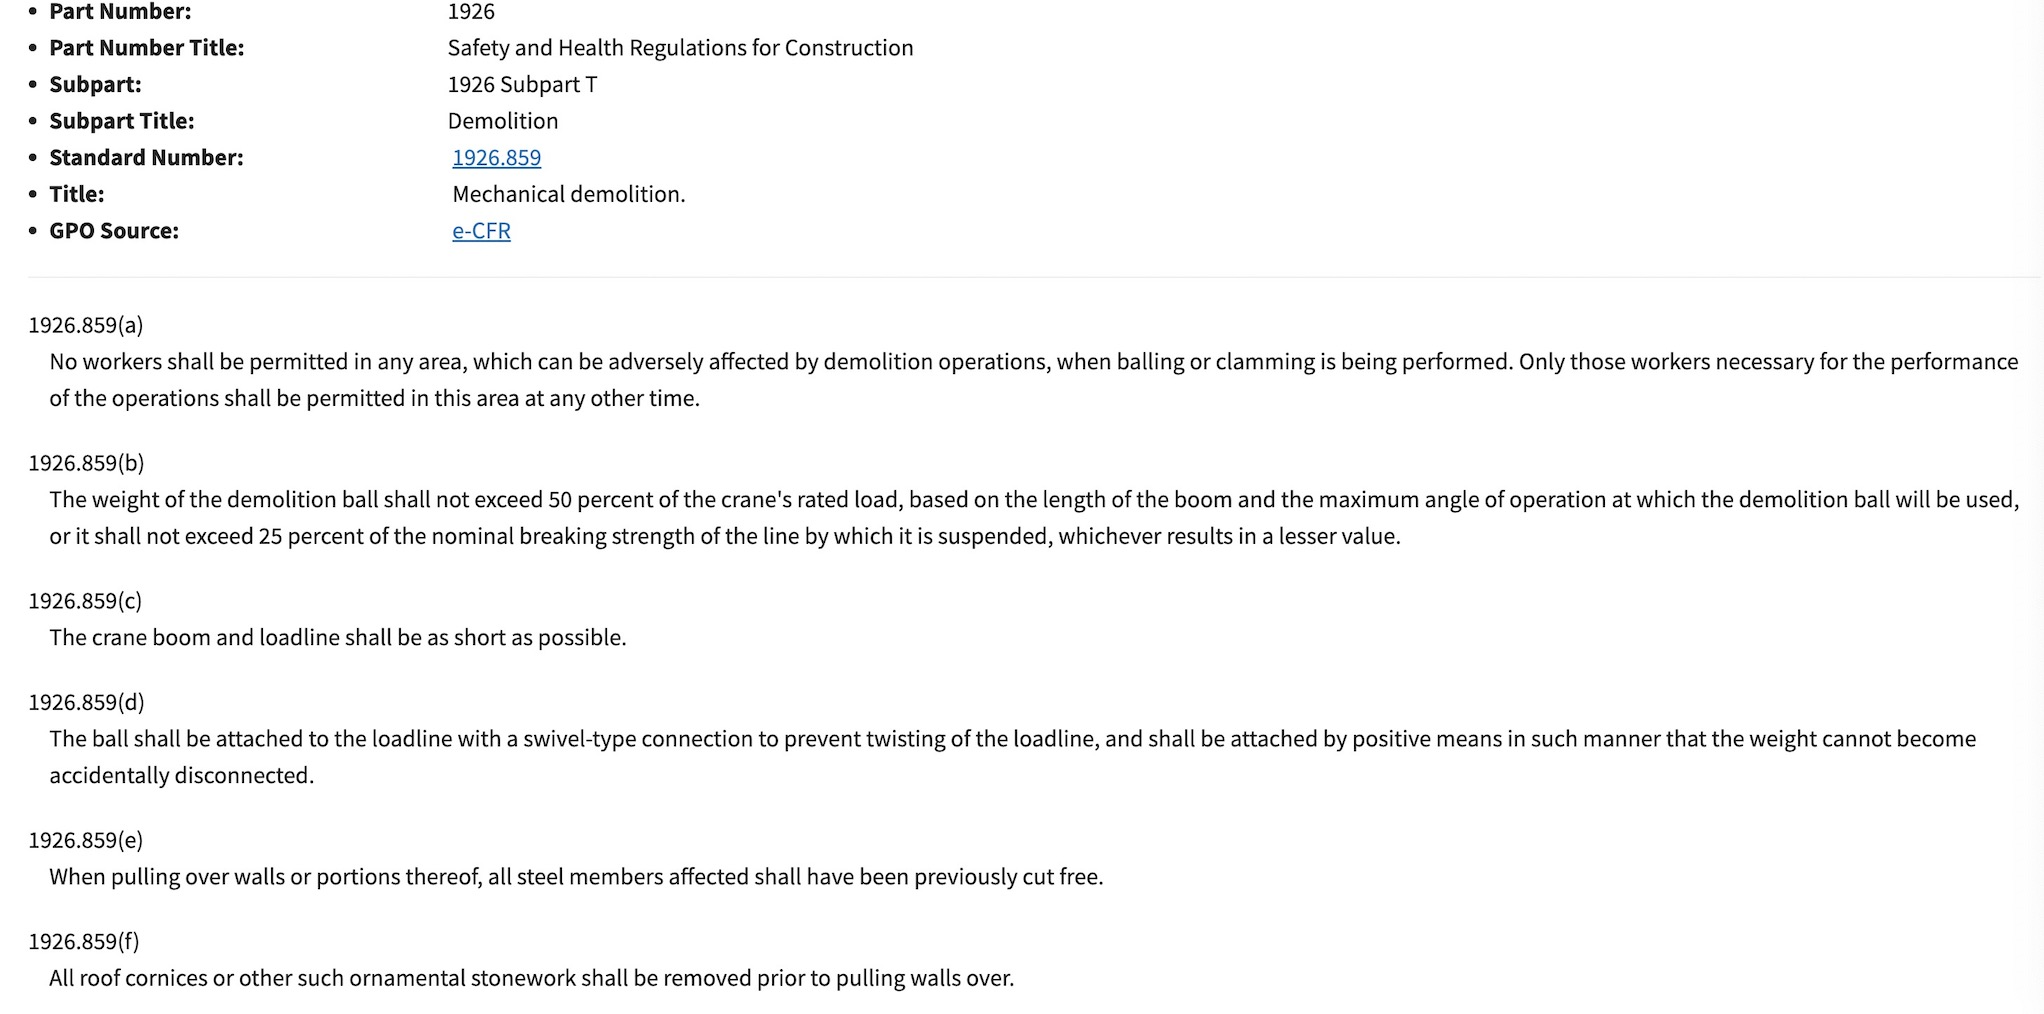
\includegraphics[width=0.5\textwidth]{figures/mechanical-demolition.jpeg}
    \caption{Regulation3}
    \label{fig:regulation3}
\end{figure}
\subsection{QA system output}
\label{sec:QA_system_output}
a figure with three images from top to bottom


\begin{figure}
    % \centering
    % \begin{subfigure}{width=0.5\textwidth}
    %     \centering
    %     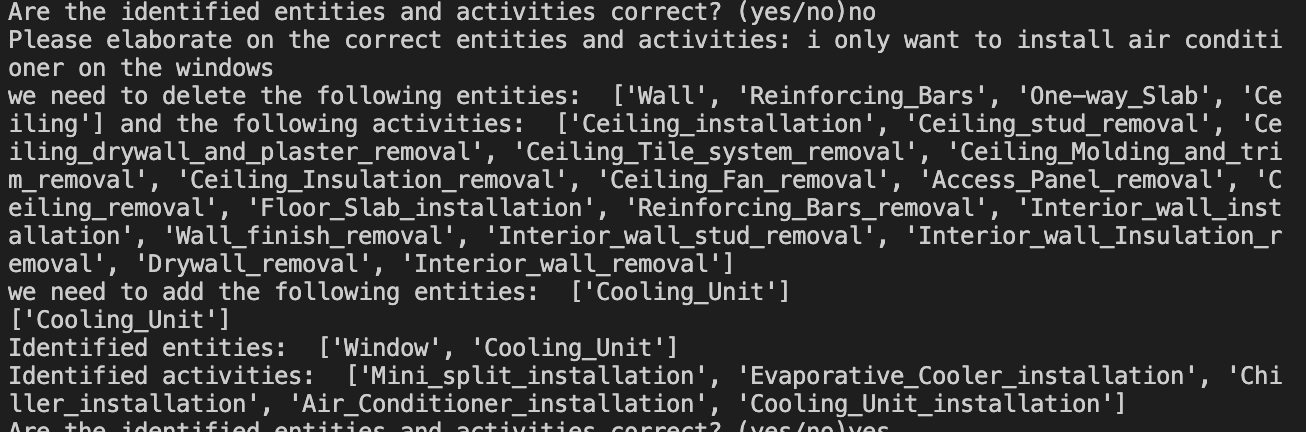
\includegraphics[width=\textwidth]{figures/sample1/step1.png}
    %     \caption{Step 1}
    %     \label{fig:output1}
    % \end{subfigure} 
    % \hfill
    % \begin{subfigure}{width=0.5\textwidth}
    %     \centering
    %     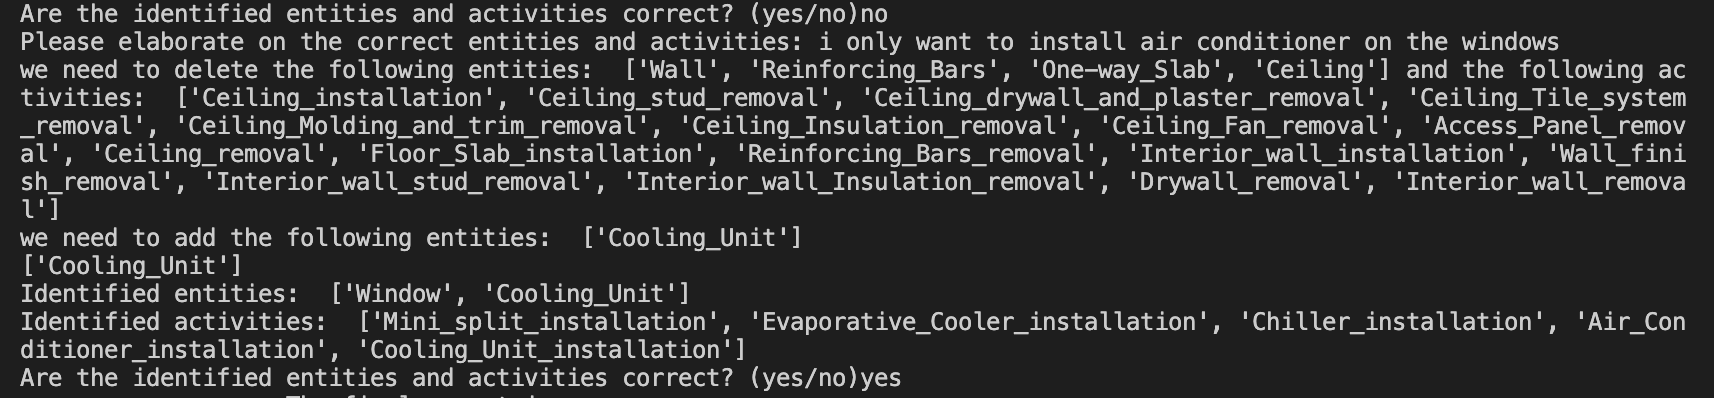
\includegraphics[width=\textwidth]{figures/sample1/step2.png}
    %     \caption{Step 2}
    %     \label{fig:output2}
    % \end{subfigure} 
    % \vfill
    % \begin{subfigure}{width=0.5\textwidth}
    %     \centering
    %     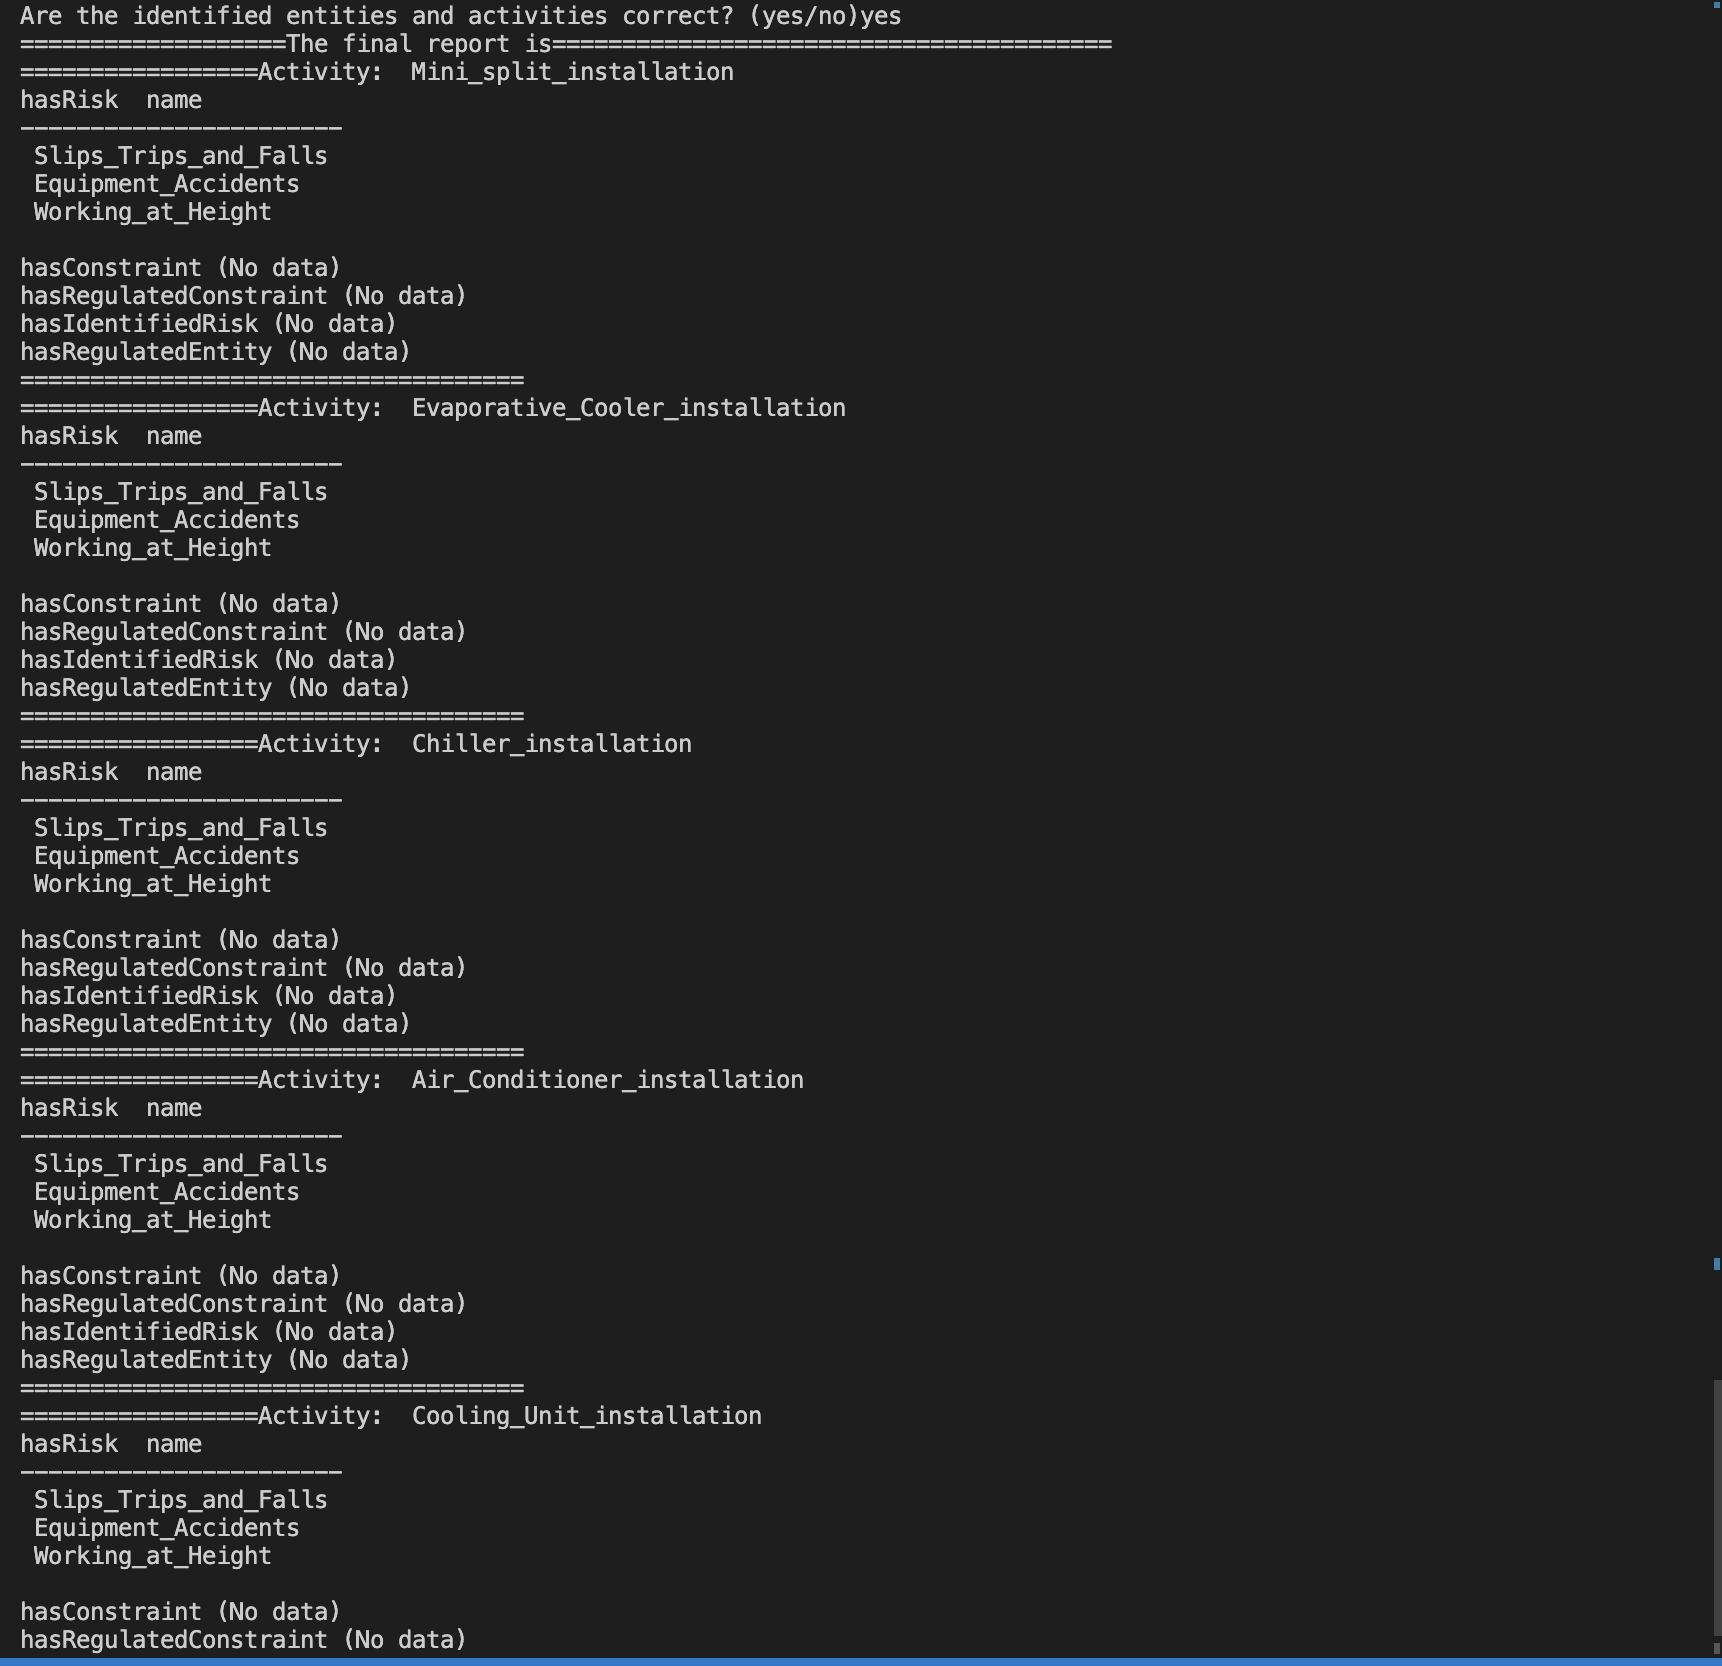
\includegraphics[width=\textwidth]{figures/sample1/step3.png}
    %     \caption{Step 3}
    %     \label{fig:output3}
    % \end{subfigure} 
    % \caption{Dialogue between the user and the system}
    % \label{fig:dialogue}
    \centering
    \subfloat[Sample1 Step 1]{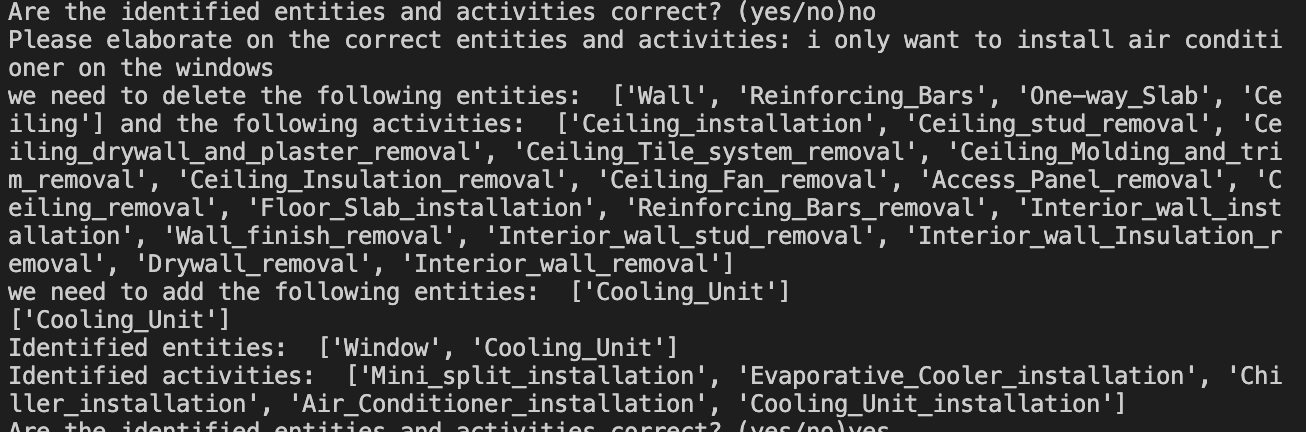
\includegraphics[width=0.4\textwidth]{figures/sample1/step1.png}\label{fig:output1}}
    \hfill
    \subfloat[Sample2 Step 1]{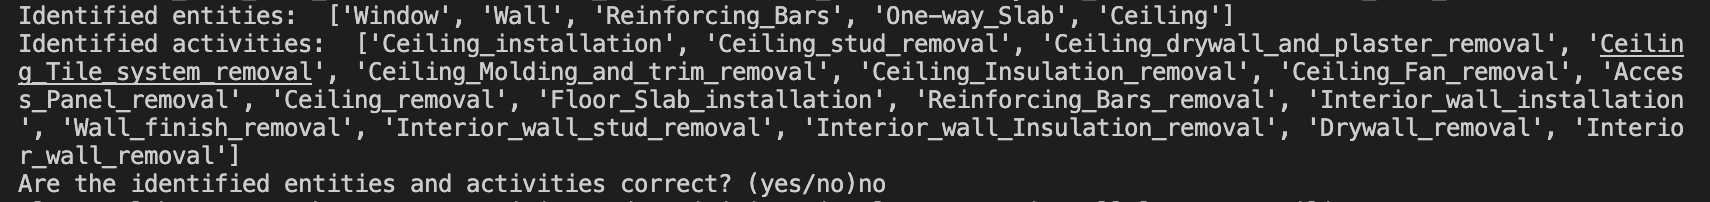
\includegraphics[width=0.4\textwidth]{figures/sample2/step1.png}\label{fig:output1.1}}
    \hfill \\
    \subfloat[Sample1 Step 2]{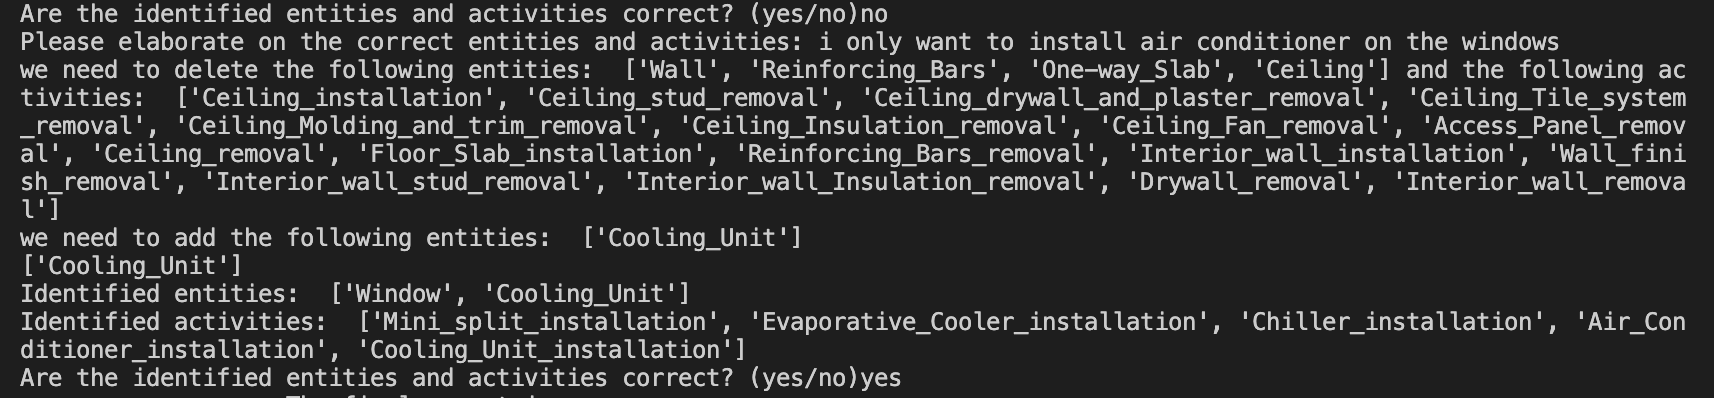
\includegraphics[width=0.4\textwidth]{figures/sample1/step2.png}\label{fig:output2}}
    \hfill
    \subfloat[Sample2 Step 1]{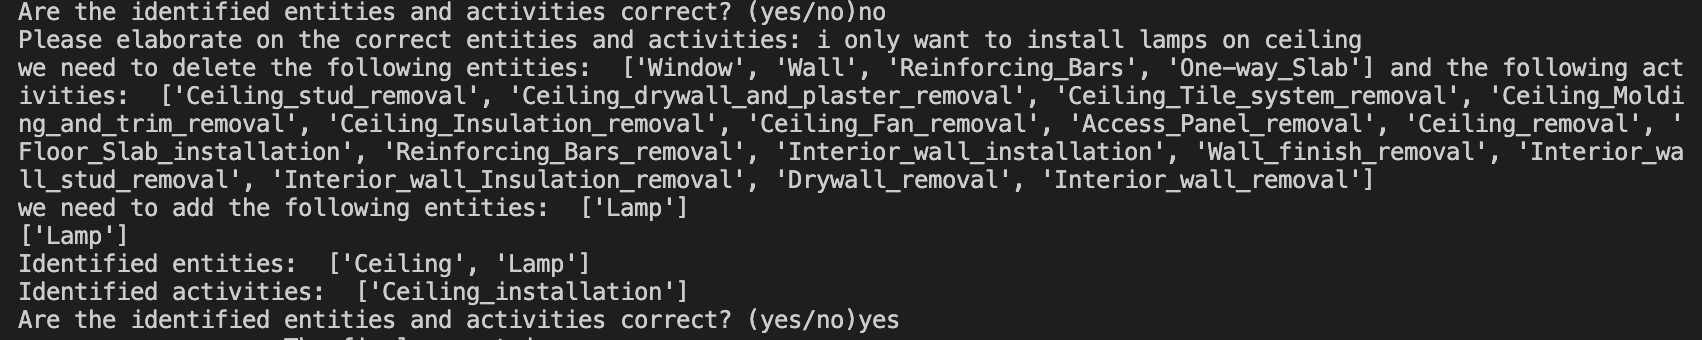
\includegraphics[width=0.4\textwidth]{figures/sample2/step2.png}\label{fig:output1.2}}
    \hfill \\
    \subfloat[Sample1 Step 3]{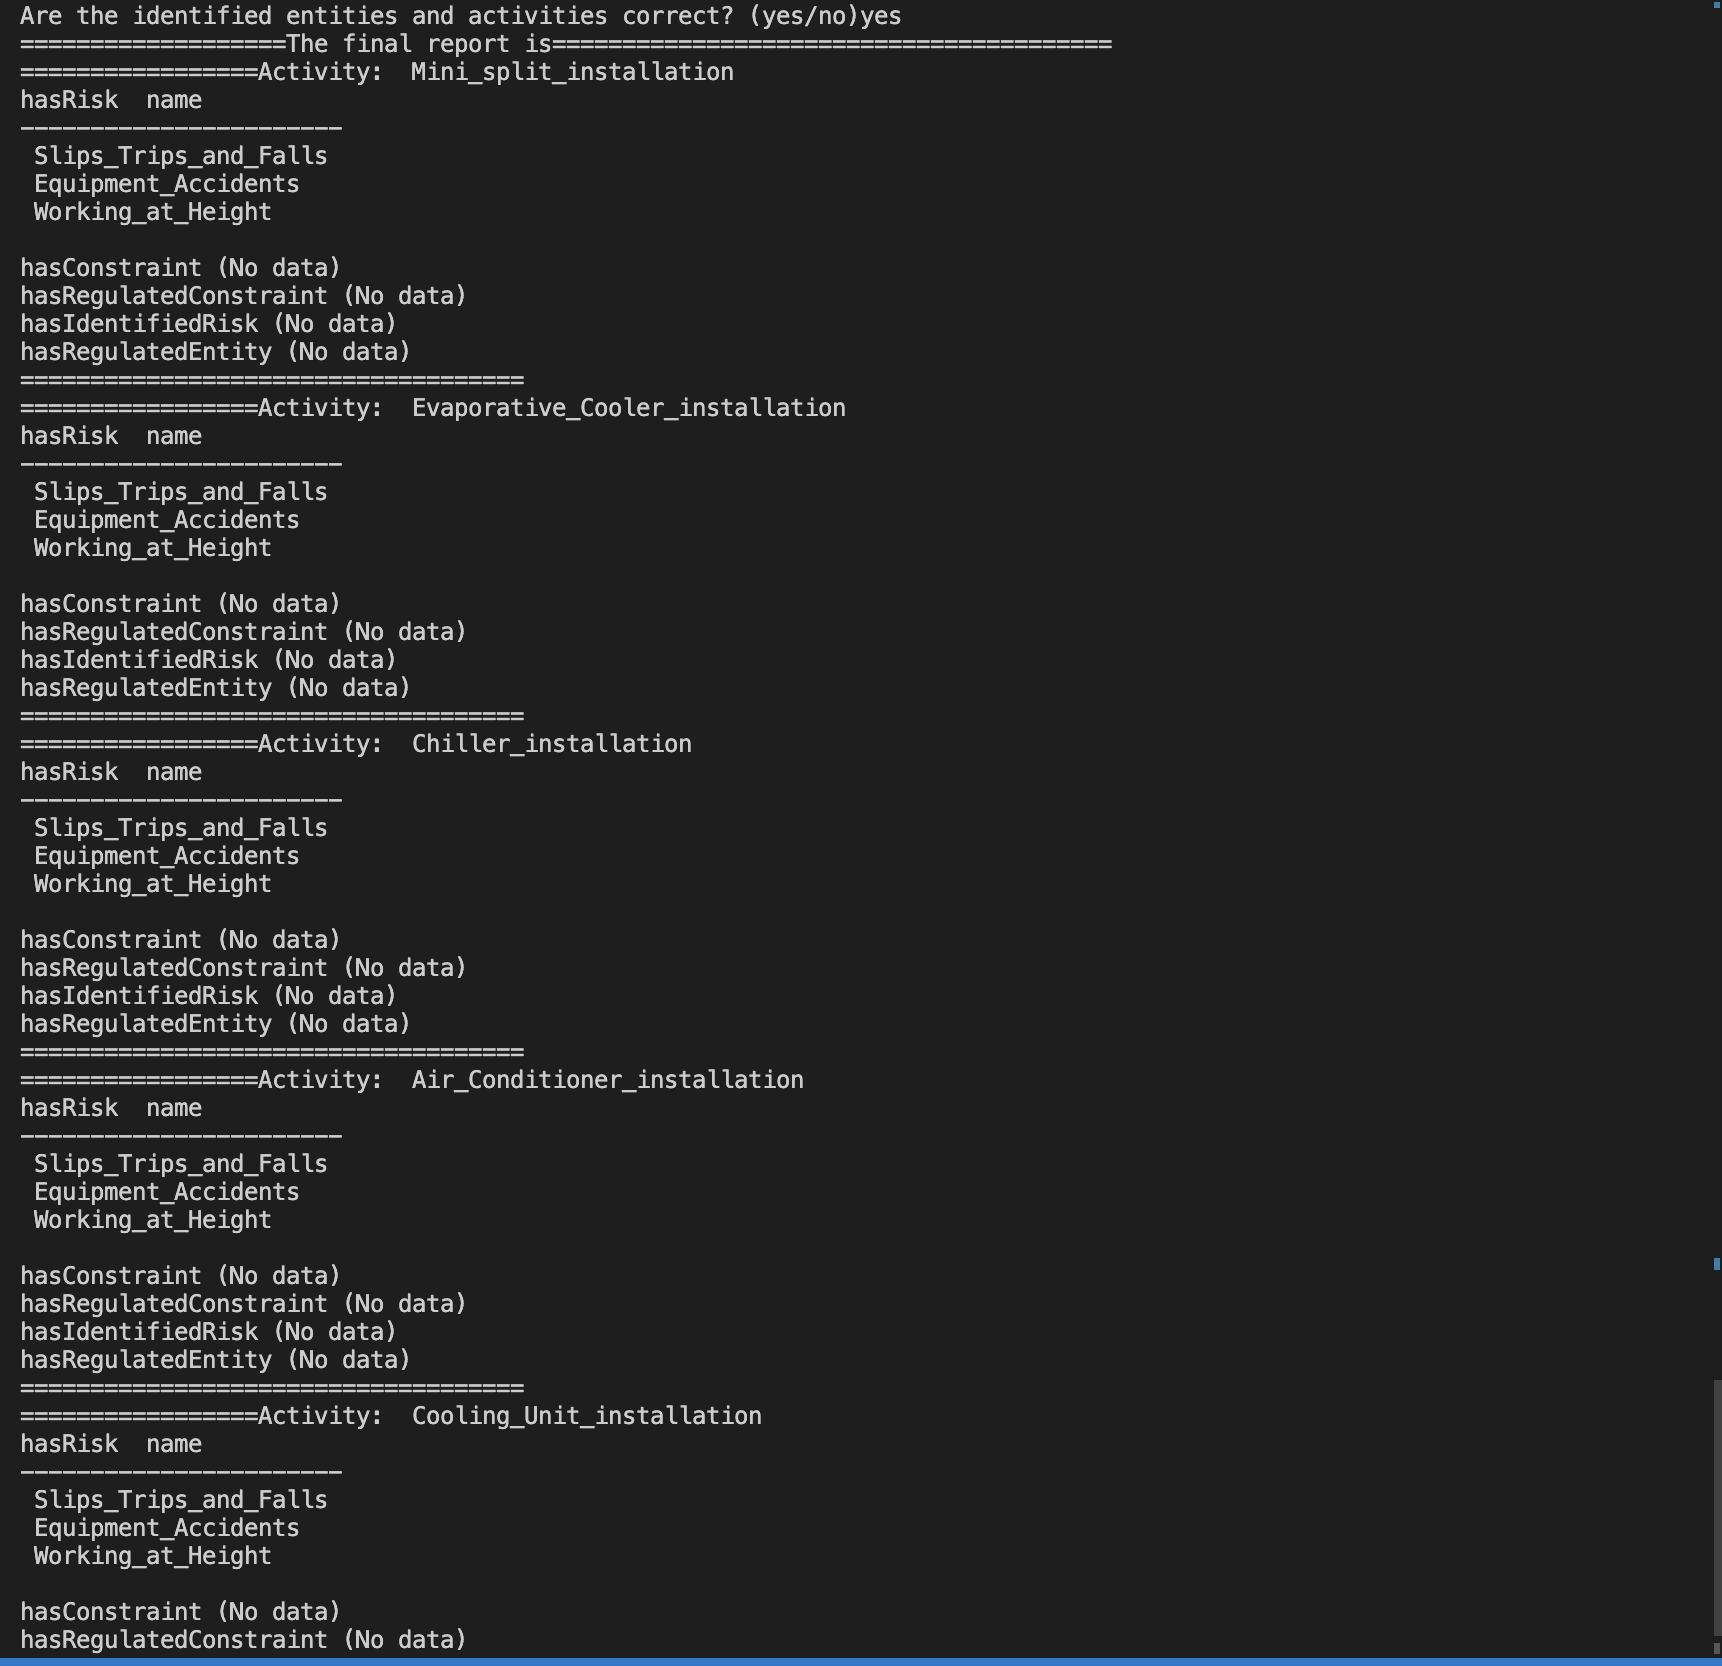
\includegraphics[width=0.4\textwidth]{figures/sample1/step3.png}\label{fig:output3}}
    \hfill
    \subfloat[Sample2 Step 1]{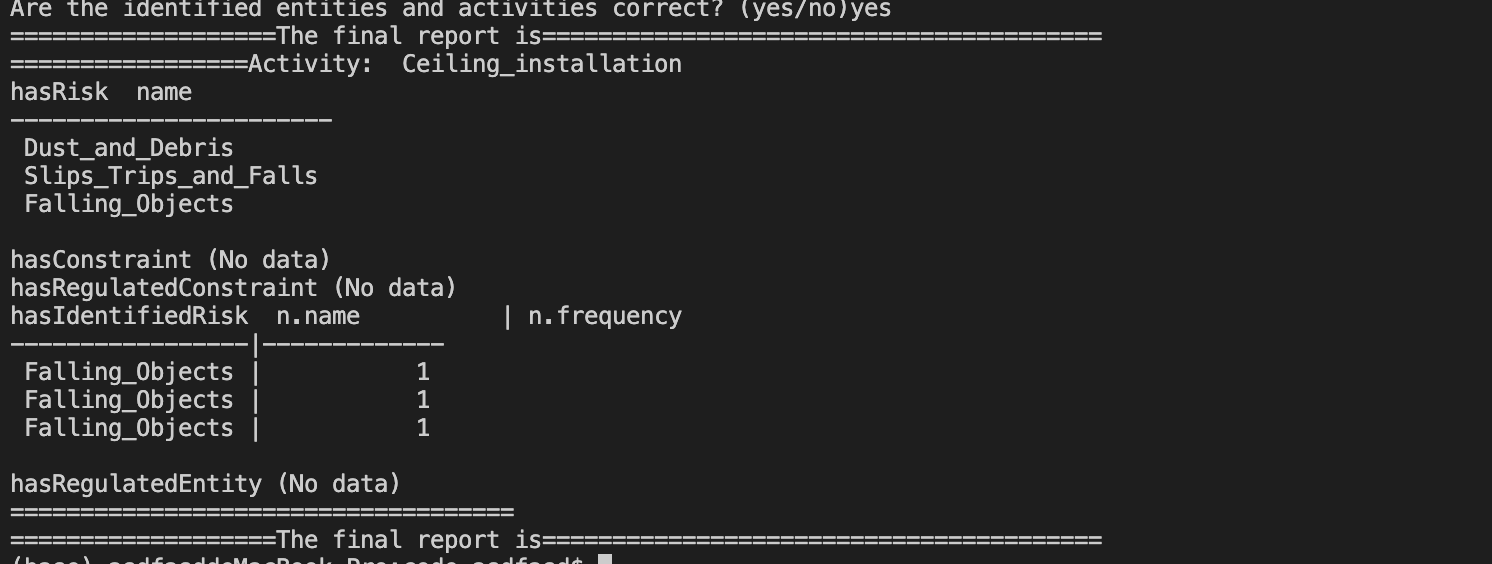
\includegraphics[width=0.4\textwidth]{figures/sample2/step3.png}\label{fig:output1.3}}
    \caption{Dialogues between the user and the system}
    \label{fig:dialouge sample}

\end{figure}




